\documentclass[tikz]{standalone}
\usepackage{amsmath}
\usepackage{color,pxfonts,fix-cm}
\usepackage{latexsym}
\usepackage{helvet}
\usepackage{lmodern}
\usepackage{fontspec}
\usepackage[T1]{fontenc}
\usepackage[utf8x]{inputenc}
\usepackage{tgpagella}
\usepackage{pict2e}
\usepackage{wasysym}
\usepackage[english]{babel}
\usepackage{tikz}
\usepackage{circuitikz}
\pagestyle{empty}
\usepackage[margin=1in]{geometry}
\usepackage{pgf}
\usepackage{pgfplots}

% Documento
\begin{document}
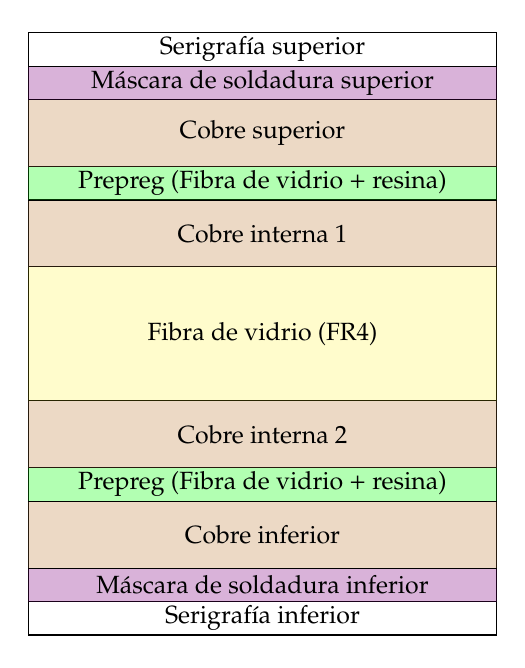
\begin{tikzpicture}[scale=0.85]
  \tikzstyle{every node}=[font=\small]
  \draw[draw=black, fill=white] (0,0) rectangle (7,0.5);
  \node at (3.5,0.25)[]{Serigrafía inferior};
  \draw(0,0.5) rectangle (7,1);
  \draw[fill=violet, opacity=0.3] (0,0.5) rectangle (7,1);
  \node at (3.5,0.75)[]{Máscara de soldadura inferior};
  \draw (0,1) rectangle (7,2);
  \draw[fill=brown, opacity=0.3] (0,1) rectangle (7,2);
  \node at (3.5,1.5)[]{Cobre inferior};
  \draw (0,2) rectangle (7,2.5);
  \draw[fill=green, opacity=0.3] (0,2) rectangle (7,2.5);
  \node at (3.5,2.25)[]{Prepreg (Fibra de vidrio + resina)};
  \draw (0,2.5) rectangle (7,3.5);
  \draw[fill=brown, opacity=0.3] (0,2.5) rectangle (7,3.5);
  \node at (3.5,3)[]{Cobre interna 2};
  \draw (0,3.5) rectangle (7,5.5);
  \draw[fill=yellow, opacity=0.2] (0,3.5) rectangle (7,5.5);
  \node at (3.5,4.5)[]{Fibra de vidrio (FR4)};
  \draw (0,5.5) rectangle (7,6.5);
  \draw[fill=brown, opacity=0.3] (0,5.5) rectangle (7,6.5);
  \node at (3.5,6)[]{Cobre interna 1};
  \draw (0,6.5) rectangle (7,7);
  \draw[fill=green, opacity=0.3] (0,6.5) rectangle (7,7);
  \node at (3.5,6.75)[]{Prepreg (Fibra de vidrio + resina)};
  \draw (0,7) rectangle (7,8);
  \draw[fill=brown, opacity=0.3] (0,7) rectangle (7,8);
  \node at (3.5,7.5)[]{Cobre superior};
  \draw (0,8) rectangle (7,8.5);
  \draw[fill=violet, opacity=0.3] (0,8) rectangle (7,8.5);
  \node at (3.5,8.25)[]{Máscara de soldadura superior};
  \draw[fill=white] (0,8.5) rectangle (7,9);
  \node at (3.5,8.75)[]{Serigrafía superior};
\end{tikzpicture}
\end{document}